\documentclass{beamer}
\usepackage[spanish]{babel}
\usepackage[latin1]{inputenc}
\usetheme{Warsaw} 
\usecolortheme{rose}
\useoutertheme{shadow}
\useinnertheme{rectangles}
\setbeamertemplate{navigation symbols}{}

\title[Modelos no Lineales para el Procesamiento de Im\'agenes]{Comparaci\'on de Modelos no Lineales para el Procesamiento de Im\'agenes}
\subtitle{Modelos no Lineales para el Procesamiento de Im\'agenes de Mamograf\'ias y Lesiones de la Piel}
\author{Carlos Toledo Silva}
\institute{Universidad de La Habana}

\date{\today}

\begin{document}
	
	\frame{\titlepage}
	
	\begin{frame}
		\frametitle{Introducci\'on}
		En la mayor�a de las circunstancias imaginables, las im�genes digitales se obtienen por medios que implican m�quinas con fuente de alimentaci�n finita; por lo tanto, las im�genes digitales se definen en un rango finito de valores. Los algoritmos de procesamiento de im�genes, tradicionalmente, se basan en operaciones reales cl�sicas para su implementaci�n. Bajo ciertas circunstancias, tal combinaci�n, denominada procesamiento lineal cl�sico de im�genes (CLIP) demuestra sus limitaciones. Por ejemplo, mencionemos el desbordamiento del rango superior e inferior, que se resuelve brutalmente mediante el truncamiento. En consecuencia, estructuras m�s elaboradas
		aparecieron, como los modelos de procesamiento logar�tmico de im�genes (LIP).
	\end{frame}
	
	\begin{frame}
		\frametitle{Introducci\'on}
		El punto de partida de los modelos logar�tmicos de procesamiento de im�genes radica en la teor�a homom�rfica introducida por Oppenheim. Las implementaciones de los modelos LIP han sido proporcionadas, seg�n nuestro mejor conocimiento, por Jourlin y Pinoli y, respectivamente, por Patrascu. Luego, el esquema de un nuevo modelo pseudo-logar�tmico fue propuesto por Vertan. Con estos modelos se han desarrollado diversas aplicaciones: correcci�n de iluminaci�n, mejora de contraste, mejora de imagen en color, ecualizaci�n de histogramas, mejora de rango din�mico, detecci�n de bordes, etc.
	\end{frame}
	
	\begin{frame}
		\frametitle{Jourlin - Pinoli Model (LIP)}
			
		\begin{block}{Dominio}
			$[0,M)$
		\end{block}
		
		\begin{block}{F\'ormula del isomorfismo}
			$\varphi(v)=-M\ln(1-\frac{v}{M})$
		\end{block}
	
		\begin{block}{Suma}
			$v_1 \oplus v_2 = v_1 + v_2 - \frac{v_1v_2}{M}$
		\end{block}
	
		\begin{block}{Resta}
			$v_1 \ominus v_2 = \frac{v_1-v_2}{1-\frac{v_2}{M}}$
		\end{block}
	
		\begin{block}{Multiplicaci\'on por escalar}
			$\lambda \otimes v = M - M(1-\frac{v}{M})^\lambda$
		\end{block}
	\end{frame}

	\begin{frame}
		\frametitle{Jourlin - Pinoli Model (LIP)}
		\begin{columns}[t]
			\column{0.5\textwidth}
			\begin{figure}[h]
				\begin{center}
					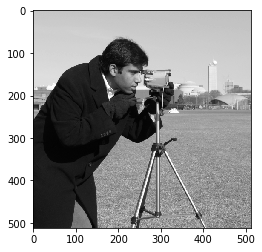
\includegraphics[width =3.0cm]{original.png}
					\caption{Imagen original}		
				\end{center}
			\end{figure}
		
			\begin{figure}[h]
				\begin{center}
					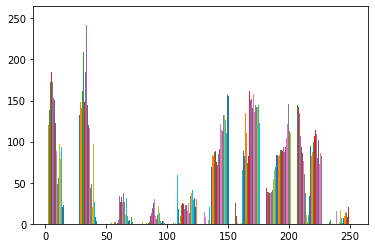
\includegraphics[width =3.0cm]{originalh.png}
					\caption{Histograma imagen original}		
				\end{center}
			\end{figure}
			
			\column{0.5\textwidth}
			\begin{figure}[h]
				\begin{center}
					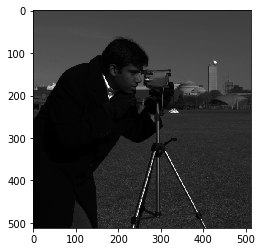
\includegraphics[width =3.0cm]{lip.png}
					\caption{Imagen en el isomorfismo}		
				\end{center}
			\end{figure}
			
			\begin{figure}[h]
				\begin{center}
					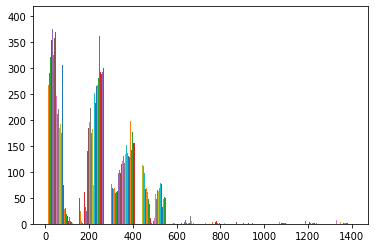
\includegraphics[width =3.0cm]{liph.png}
					\caption{Histograma en isomorfismo}		
				\end{center}
			\end{figure}
		\end{columns}
	\end{frame}

	\begin{frame}
		\frametitle{SLIP}
		\begin{block}{Dominio}
			$(-M,M)$
		\end{block}
		
		\begin{block}{F\'ormula del isomorfismo}
			$\varphi(v)=-M sgn(v)\ln(1-\frac{|v|}{M})$
		\end{block}
		
		\begin{block}{Suma}
			$v_1 \oplus v_2 = M sgn(v_1+v_2)[1-(1-\frac{|v_1|}{M})^{\gamma_1}(1-\frac{|v_2|}{M})^{\gamma_2}],~~\gamma_1=\frac{sgn(v_1)}{sgn(v_1+v_2)}$
			
			$\gamma_2=\frac{sgn(v_2)}{sgn(v_1+v_2)}$
			
		\end{block}
		
		\begin{block}{Resta}
			$v_1 \ominus v_2 = v_1 \oplus (-1 \otimes v_2)$
		\end{block}
		
		\begin{block}{Multiplicaci\'on por escalar}
			$\lambda \otimes v = Msgn(\lambda v)[1-(1-\frac{|v|}{M})^{|\lambda|}]$
		\end{block}
	\end{frame}
	
	\begin{frame}
		\frametitle{SLIP}
		\begin{columns}[t]
			\column{0.5\textwidth}
			\begin{figure}[h]
				\begin{center}
					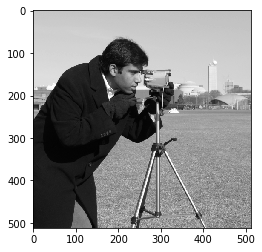
\includegraphics[width =3.0cm]{original.png}
					\caption{Imagen original}		
				\end{center}
			\end{figure}
			
			\begin{figure}[h]
				\begin{center}
					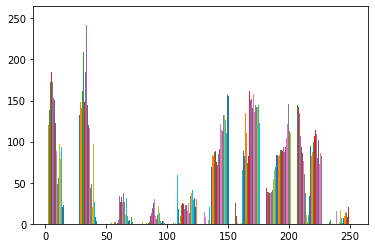
\includegraphics[width =3.0cm]{originalh.png}
					\caption{Histograma imagen original}		
				\end{center}
			\end{figure}
			
			\column{0.5\textwidth}
			\begin{figure}[h]
				\begin{center}
					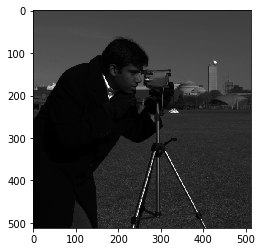
\includegraphics[width =3.0cm]{slip.png}
					\caption{Imagen en el isomorfismo}		
				\end{center}
			\end{figure}
			
			\begin{figure}[h]
				\begin{center}
					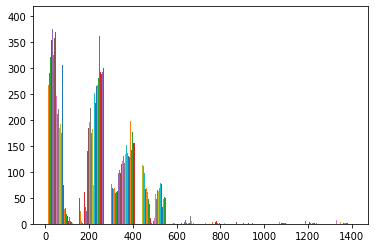
\includegraphics[width =3.0cm]{sliph.png}
					\caption{Histograma en isomorfismo}		
				\end{center}
			\end{figure}
		\end{columns}
	\end{frame}

	\begin{frame}
		\frametitle{Patrascu Model}
		\begin{block}{Dominio}
			$[0,M)$
		\end{block}
		
		\begin{block}{F\'ormula del isomorfismo}
			$\varphi(v)=\frac{M}{4}\ln(\frac{x}{1-x}), x=\frac{v+1}{M+1}$
		\end{block}
		
		\begin{block}{Suma}
			$v_1 \oplus v_2 = (M+1) \frac{x_1x_2}{(1-x_1)(1-x_2)-x_1x_2}-1, x_1=\frac{v_1+1}{M+1},x_2=\frac{v_2+1}{M+1}$
		\end{block}
		
		\begin{block}{Resta}
			$v_1 \ominus v_2 = (M+1) \frac{x_1(1-x_2)}{(1-x_1)x_2+(1-x_2)x_1}-1, x_1=\frac{v_1+1}{M+1},x_2=\frac{v_2+1}{M+1}$
		\end{block}
		
		\begin{block}{Multiplicaci\'on por escalar}
			$\lambda \otimes v = (M+1)\frac{x^\lambda}{x^\lambda+(1-x)^\lambda}-1, x=\frac{v+1}{M+1}$
		\end{block}
	\end{frame}
	

	\begin{frame}
		\frametitle{Patrascu Model}
		\begin{columns}[t]
			\column{0.5\textwidth}
			\begin{figure}[h]
				\begin{center}
					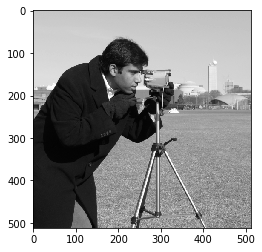
\includegraphics[width =3.0cm]{original.png}
					\caption{Imagen original}		
				\end{center}
			\end{figure}
			
			\begin{figure}[h]
				\begin{center}
					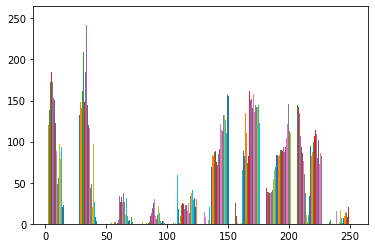
\includegraphics[width =3.0cm]{originalh.png}
					\caption{Histograma imagen original}		
				\end{center}
			\end{figure}
			
			\column{0.5\textwidth}
			\begin{figure}[h]
				\begin{center}
					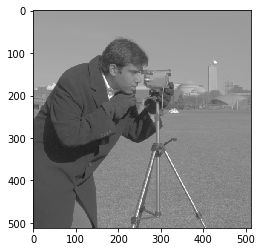
\includegraphics[width =3.0cm]{patrascu.png}
					\caption{Imagen en el isomorfismo}		
				\end{center}
			\end{figure}
			
			\begin{figure}[h]
				\begin{center}
					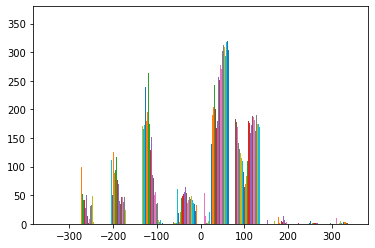
\includegraphics[width =3.0cm]{patrascuh.png}
					\caption{Histograma en isomorfismo}		
				\end{center}
			\end{figure}
		\end{columns}
	\end{frame}
	
	\begin{frame}
		\frametitle{Vertan Model (Pseudo-logarithmic Model)}
		\begin{block}{Dominio}
			$[0,M)$
		\end{block}
		
		\begin{block}{F\'ormula del isomorfismo}
			$\varphi(v)=M\frac{v}{M-v}$
		\end{block}
		
		\begin{block}{Suma}
			$v_1 \oplus v_2 = M \frac{x_1+x_2-2x_1x_2}{1-x_1x_2},x_1=\frac{v_1}{M}~x_2=\frac{v_2}{M}$
		\end{block}
		
		\begin{block}{Resta}
			$v_1 \ominus v_2 = M \frac{x_1-x_2}{1+x_1x_2-2x_2},x_1=\frac{v_1}{M}~x_2=\frac{v_2}{M}$
		\end{block}
		
		\begin{block}{Multiplicaci\'on por escalar}
			$\lambda \otimes v = M\frac{\lambda x}{1-(\lambda-1)x},x=\frac{v}{M}$
		\end{block}
	\end{frame}
	
	
	\begin{frame}
		\frametitle{Vertan Model (Pseudo-logarithmic Model)}
		\begin{columns}[t]
			\column{0.5\textwidth}
			\begin{figure}[h]
				\begin{center}
					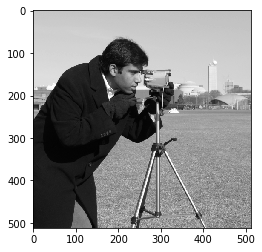
\includegraphics[width =3.0cm]{original.png}
					\caption{Imagen original}		
				\end{center}
			\end{figure}
			
			\begin{figure}[h]
				\begin{center}
					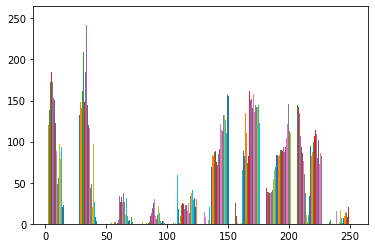
\includegraphics[width =3.0cm]{originalh.png}
					\caption{Histograma imagen original}		
				\end{center}
			\end{figure}
			
			\column{0.5\textwidth}
			\begin{figure}[h]
				\begin{center}
					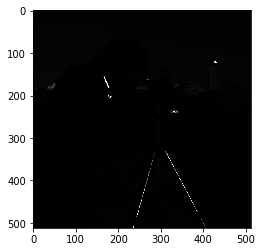
\includegraphics[width =3.0cm]{plipf.png}
					\caption{Imagen en el isomorfismo}		
				\end{center}
			\end{figure}
			
			\begin{figure}[h]
				\begin{center}
					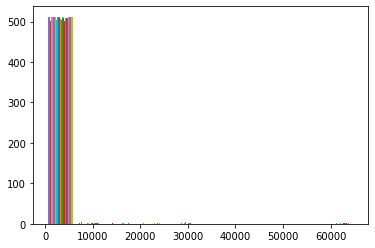
\includegraphics[width =3.0cm]{plipfh.png}
					\caption{Histograma en isomorfismo}		
				\end{center}
			\end{figure}
		\end{columns}
	\end{frame}
	
\end{document}